\let\negmedspace\undefined
\let\negthickspace\undefined
\documentclass[journal]{IEEEtran}
\usepackage[a5paper, margin=10mm, onecolumn]{geometry}
\usepackage{lmodern} % Ensure lmodern is loaded for pdflatex
\usepackage{tfrupee} % Include tfrupee package

\setlength{\headheight}{1cm} % Set the height of the header box
\setlength{\headsep}{0mm}     % Set the distance between the header box and the top of the text

\usepackage{gvv-book}
\usepackage{gvv}
\usepackage{cite}
\usepackage{amsmath,amssymb,amsfonts,amsthm}
\usepackage{algorithmic}
\usepackage{graphicx}
\usepackage{textcomp}
\usepackage{xcolor}
\usepackage{txfonts}
\usepackage{listings}
\usepackage{enumitem}
\usepackage{mathtools}
\usepackage{gensymb}
\usepackage{comment}
\usepackage[breaklinks=true]{hyperref}
\usepackage{tkz-euclide} 
\usepackage{listings}                                      
\def\inputGnumericTable{}                                 
\usepackage[latin1]{inputenc}                                
\usepackage{color}                                            
\usepackage{array}                                            
\usepackage{longtable}
\usepackage{multicol}
\usepackage{calc}                                             
\usepackage{multirow}                                         
\usepackage{hhline}                                           
\usepackage{ifthen}                                           
\usepackage{lscape}
\begin{document}
	
	\bibliographystyle{IEEEtran}
	\vspace{3cm}
	
	\title{10.4.2.5}
	\author{EE24BTECH11064 - Harshil Rathan}
	% \maketitle
	% \newpage
	% \bigskip
	{\let\newpage\relax\maketitle}
	
	\renewcommand{\thefigure}{\theenumi}
	\renewcommand{\thetable}{\theenumi}
	\setlength{\intextsep}{10pt} % Space between text and floats
	
	
	\numberwithin{equation}{enumi}
	\numberwithin{figure}{enumi}
	\renewcommand{\thetable}{\theenumi}
	
	
\textbf{Question}:\\
The altitude of a right triangle is 7cm less than its base. If the hypotenuse is 13cm, find the other two sides 
\\
\textbf{Solution: }\\
We get the equation 
\begin{align}
    x^2 + (x-7)^2 = 13^2 
\end{align}
\begin{align}
     x^2-7x-60 =0
\end{align}
We can solve the above equation using fixed point iterations. First we separate $x$, from the above equation and make an update equation of the below sort.
\begin{align}
	x = g\brak{x} = \frac{x^2-60}{7}
\end{align}
Applying the above update equation on our equation, we get
\begin{align}
	x_{n+1}=\frac{x_n^2-60}{7}
\end{align}
Now we start with an initial guess $x_0 = 10 $\\
 But we realize that the updated values always approach infinity for any initial value. \\
Thus we will alternatively use Newton's Method for solving equations.
\begin{align}
	x_{n+1} = x_n - \frac{f\brak{x_n}}{f^{\prime}\brak{x_n}} 
\end{align}
Where we define $f\brak{x}$ as, 
\begin{align}
	f(x) = x^2 - 7x - 60 
\end{align}
\begin{align}
    f'(x) = 2x - 7
\end{align}
Thus, the new update equation is, 
\begin{align}
	x_{n+1} = x_n - \frac{x_n^2-7x_n-60}{2x_n-7 } 
\end{align}
Taking the initial guess as $x_0 = 10$, we can see that $x_n$ converges with x as,
\begin{align}
	x \approx 12.002
\end{align}
\begin{align}
    x = 12cm 
\end{align}
Alternatively, we can use the Secant method for solving equations.
\begin{align}
	x_{n+1} = x_n + f\brak{x_n}\frac{x_{n} -  x_{n-1}}{f(x_{n}) -  f(x_{n-1})}
\end{align}
The altitude is 
\begin{align}
    12 - 7 = 5cm 
\end{align}
\textbf{Solution using Eigenvalue approach}\\
Alternatively we use QR decomposition to find eigenvalues\\
We say a matrix $A$ is in hessenberg form if it is in form shown below
\begin{align}
H = 
\myvec{
\times & \times & \times & \cdots & \times \\
\times & \times & \times & \cdots & \times \\
0      & \times & \times & \cdots & \times \\
0      & 0      & \times & \cdots & \times \\
\vdots & \vdots & \vdots & \ddots & \vdots \\
0      & 0      & 0      & \cdots & \times
}
\end{align}
We will use householder method to reduce any matrix into hessenberg form.\\
It reduces an $n\times n$ matrix to hessenberg form by $n-2$ orthogonal trasformations. Each transformations annihilates the required part of a whole column at a time rather than element wise elimination. The basic ingredient for a house holder matrix is $P$ which is in the form
\begin{align}
	P = I-2\vec{w}\vec{w}^\top
\end{align}
where w is a vector with $\abs{w}^2=1$. The matrix $P$ is orthogonal as
\begin{align}
P^2 &=\brak{I - 2\vec{w}\vec{w}^\top}\cdot\brak{I - 2\vec{w}\vec{w}^\top}\\
    &=I-4\vec{w}\vec{w}^\top + 4\vec{w}\cdot\brak{\vec{w}^\top\vec{w}^\top}\cdot\vec{w}^\top\\
    &=I
\end{align}
Therefore, $P=P^{-1}$ but $P = P^\top$, so $P = P^\top$ \\
We can rewrite $P$ as
\begin{align}
	P = I - \frac{\vec{u}\vec{u}^\top}{H}
\end{align}
where the scalar $H$ is
\begin{align}
H = \frac{1}{2}\abs{\vec{u}}^2
\end{align}
Where $\vec{u}$ can be any vector. Suppose $\vec{x}$ is the vector composed of the first column of $A$. Take
\begin{align}
	\vec{u} = \vec{x} \mp \abs{\vec{x}}\vec{e}_1
\end{align}
Where $\vec{e}_1 = \myvec{1 & 0 & \dots}^\top$, we will take the choice of sign later. Then
\begin{align}
	P\cdot\vec{x} &= \vec{x} - \frac{\vec{u}}{H}\cdot\brak{\vec{u}\mp \abs{\vec{x}}\vec{e}_1}^\top\cdot \vec{x}\\
	              &= \vec{x} - \frac{2\vec{u}\brak{\abs{x}^2\mp \abs{x}x_1}}{2\abs{x}^2\mp \abs{x}x_1}\\
	              &= \vec{x} - \vec{u}\\
	              &= \mp\abs{\vec{x}}\vec{e}_1
\end{align}
To reduce a matrix $A$ into Hessenberg form, we choose vector $\vec{x}$ for the first householder matrix to be lower $n-1$ elements of the first column, then the lower $n-2$ elements will be zeroed.
\begin{align}
P_1\cdot A &= \myvec{
1 & 0 & 0 & \cdots & 0 \\
0 & p_{11} & p_{12} & \cdots & p_{1n} \\
0      & p_{21} & p_{22} & \cdots & p_{2n} \\
0      & p_{31} & p_{32} & \cdots & p_{3n} \\
\vdots & \vdots & \vdots & \ddots & \vdots \\
0      & p_{n1} & p_{n2} & \cdots & p_{nn}
}\myvec{
a_{00} & \times & \times & \cdots & \times \\
a_{10} & \times & \times & \cdots & \times \\
a_{20} & \times & \times & \cdots & \times \\
a_{30} & \times & \times & \cdots & \times \\
\vdots & \vdots & \vdots & \ddots & \vdots \\
a_{n0} & \times & \times & \cdots & \times
}\\
&=\myvec{
a_{00}^\prime & \times & \times & \cdots & \times \\
0 & \times & \times & \cdots & \times \\
0      & \times & \times & \cdots & \times \\
0      & \times   & \times & \cdots & \times \\
\vdots & \vdots & \vdots & \ddots & \vdots \\
0      & \times      & \times      & \cdots & \times
}
\end{align}
Now if we multiply the matrix $P_1A$ with $P_1$, the eigenvalues will be conserved as it is a similarity transformation.\\
Now we choose the vector $\vec{x}$ for the householder matrix to be the bottom $n-2$ elements of the second column, and from it construct the $P_2$
\begin{align}
P_2 = \myvec{
1 & 0 & 0 & \cdots & 0 \\
0 & 1 & 0 & \cdots & 0 \\
0 & 0 & p_{22} & \cdots & p_{2n} \\
0 & 0 & p_{32} & \cdots & p_{3n} \\
\vdots & \vdots & \vdots & \ddots & \vdots \\
0 & 0 & p_{n2} & \cdots & p_{nn}
}
\end{align}
Now if do similarity transform $PAP$, we will zero out the $n-3$ elements in second column.
If we continue this pattern we will get the hessenberg form of a the matrix $A$.
In this algorithm, we decompose matrix given in Hessenberg form to two matrices $Q$ and $R$ such that $Q$ is an orthogonal matrix and $R$ is an upper triangular matrix. Then we assign the new matrix $A^\prime$ to be $A^\prime = RQ$, and we do this iteratively. Theoritically, as the number of iterations go to infinite, the matrix $A^\prime$ will converge to an upper triangular matrix whose diagonal elements are the eigenvalues of $A$. There will be a minor problem in this method when the entries are real while the eigenvalues are complex, we will solve this issue shortly. The eigenvalues of the matrix $A$ will not change because of the following
\begin{align}
	A &= QR\\
	R &= Q^\top A\\
	A^\prime &= RQ\\
	A^\prime &= Q^\top AQ
\end{align}
As the matrix $A$ is undergoing similarity transformation, the eigenvalues will not change.\\
The rate of covergence of $A$ depends on the ratio of absolute values of the eigenvalues. That is, if the eigenvalues are $\abs{\lambda_1} \geq \abs{\lambda_2} \geq \abs{\lambda_3} \dots \geq \abs{\lambda_n}$ then, the elements of $A_k$ below the diagonal to converge to zero like
\begin{align}
    \abs{a_{ij}^{\brak{k}}} = O\brak{\abs{\frac{\lambda_i}{\lambda_j}}^k}\text{    } i > j
\end{align}
\\
The QR decomposition is implemented using the Givens rotation technique. This approach is robust and numerically stable, making it ideal for QR decomposition, especially in iterative methods like eigenvalue computations. It is every similar to Jacobian Transformation. We define a rotation matrix $G$, to zero out the elements which are non-diagonal, since the matrix which we are dealing is a Hessenberg matrix, we need to zero out the elements which are just below the diagonal elements.
\begin{align}
G = \myvec{
1 & \cdots & 0 & 0 & \cdots & 0 \\
\vdots & \ddots & \vdots & \vdots & \reflectbox{$\ddots$} & \vdots \\
0 & \cdots & c & s & \cdots & 0\\
0 & \cdots & -s & c & \cdots & 0\\
\vdots & \reflectbox{$\ddots$} & \vdots & \vdots & \ddots & \vdots\\
0 & \cdots & 0 & 0 & \cdots & 1
}
\end{align}
Where the value of $c$ and $s$ are
\begin{align}
	c = \frac{\overline{x_{i,i}}}{\sqrt{\abs{x_{i,i}}^2+\abs{x_{i,i+1}}^2}}\\
	s = \frac{\overline{x_{i,i+1}}}{\sqrt{\abs{x_{i,i}}^2+\abs{x_{i,i+1}}^2}}
\end{align}
If we multiply $G$ and $A$, we can see easily that it nulls out the element in $\brak{i+1}^{\text{th}}$ row and $i^\text{th}$ column. The following matrix multiplication eliminates all the elements below the diagonal of $A$
\begin{align}
	A \implies G_{n-1}G_{n-2}\cdots G_2G_1A
\end{align}
Now, we store $G_{n-1}G_{n-2}\cdots G_2G_1$ in $Q$ and then
\begin{align}
	A^\prime \implies QAQ^\top\\
\end{align}
If we carry out these transformation infinite times, the $A$ will be an upper triangular matrix with diagonal elements as eigenvalues.
If all the entries in the matrix are real but the eigenvalues are complex, the matrix $A$ will converge to a Quasi-triangular form, that is
\begin{align}
	A = \myvec{B_1 & 0 & \cdots & 0 \\
		   0 & B_2 & \cdots & 0\\
		   \vdots & \cdots & \ddots & 0\\
		   0 & 0 & 0 & B_n}
\end{align}
Where $B_i$ is a $2 \times 2$ block matrix. These matrices are called jordan blocks. In this case, the eigenvalues are calculated by solving the characteristic equation of the $2 \times 2$ matrix. Since it will be a quadratic equation, it can be easily solved and the solutions of that characteristic equation will be the eigenvalues.\newline
The major defect in QR decomposition algorithm is that sometimes the rate of convergence is very low. The idea behind Rayleigh Quotient method is really simple, since the rate of convergence is low, we will increase the rate of convergence by making a shift. According to the order of rate of covergence given in equation \brak{0.35}, if null of the last element \brak{\lambda_i=0} the order of convergence will be very high. So what we do is we shift the Hessenberg matrix by some amount, apply QR decomposition algorithm and add the shift back. If this shift is exactly the eigenvalue then it completes in very less number of iteration (best case, only 1 iteration). But since we do not know the eigenvalue, we will take the guess to be the last diagonal element.
\begin{align}
	H^\prime &= H - \sigma I\\
	H^\prime &\implies {H^\prime}_{tranformed}\\
	H_{next} &= {H^\prime}_{tranformed} + \sigma I
\end{align}
This method does not change the eigenvalues as
\begin{align}
\overline{H} &= Q\brak{H - \lambda I}Q^\top\\
	&= QHQ^\top - \lambda QIQ^\top\\
	&= QHQ^\top - \lambda I\\
\overline{H} +\lambda I &= QHQ^\top
\end{align}
which is a similarity tranformation.\\
Here, once we finding the eigenvalue and it is in the last diagonal element, we will leave it as it is and then focus on smaller matrix block present diagonally above the eigenvalue and then use the same technique to push the next eigenvalue to the next diagonal element. We will continue to do this till all the eigenvalues are present in the diagonal. This is know as deflation.
\begin{align}
H  - \lambda I = QR\\
R = \myvec{\times & \times & \cdots & \times\\
	0 & \times & \cdots & \times\\
	\vdots & \vdots & \ddots & \times\\
	0 & 0 & \cdots & 0}
\end{align}
$RQ$ Will also be in the same form
\begin{align}
\overline{H} = RQ+\lambda I = \myvec{\overline{H_1} & \vec{h}_1\\0^\top & \lambda}
\end{align}
The companion matrix for the quadratic equation $x^2 - 7x - 60 = 0$ is:
\begin{align}
    H = \begin{bmatrix}
        7 & 60 \\
        1 & 0
    \end{bmatrix}.
\end{align}

Since $H$ is already in Hessenberg form, we can directly proceed with the QR iteration. For the first iteration:
\begin{align}
    \sigma &= H_{2,2} = 0, \\
    H_{\text{shifted}} &= H - \sigma I = \begin{bmatrix}
        7 & 60 \\
        1 & 0
    \end{bmatrix}.
\end{align}

The Givens rotation parameters are calculated as:
\begin{align}
    x_{1,1} &= 7, \\
    x_{2,1} &= 1, \\
    c &= \frac{x_{1,1}}{\sqrt{x_{1,1}^2 + x_{2,1}^2}} = \frac{7}{\sqrt{7^2 + 1^2}} \approx 0.989949, \\
    s &= \frac{x_{2,1}}{\sqrt{x_{1,1}^2 + x_{2,1}^2}} = \frac{1}{\sqrt{7^2 + 1^2}} \approx 0.141421.
\end{align}

The Givens rotation matrix $Q$ is:
\begin{align}
    Q = \begin{bmatrix}
        c & s \\
        -s & c
    \end{bmatrix}
    = \begin{bmatrix}
        0.989949 & 0.141421 \\
        -0.141421 & 0.989949
    \end{bmatrix}.
\end{align}

Next, compute $R$ and update $H$:
\begin{align}
    R &= QH_{\text{shifted}}, \\
    H_{\text{new}} &= RQ.
\end{align}

After iterating for 20 steps, the matrix converges to:
\begin{align}
    H = \begin{bmatrix}
        -5 & 0 \\
        0 & 12
    \end{bmatrix}.
\end{align}

Thus, the eigenvalues (and roots of the quadratic equation) are:
\begin{align}
    \lambda_1 = -5, \quad \lambda_2 = 12.
\end{align}
We get the eigenvalues as 12 and -5\\ 
The base is 12cm and the altitude is 5cm 
	\begin{figure}[h!]
		\centering
		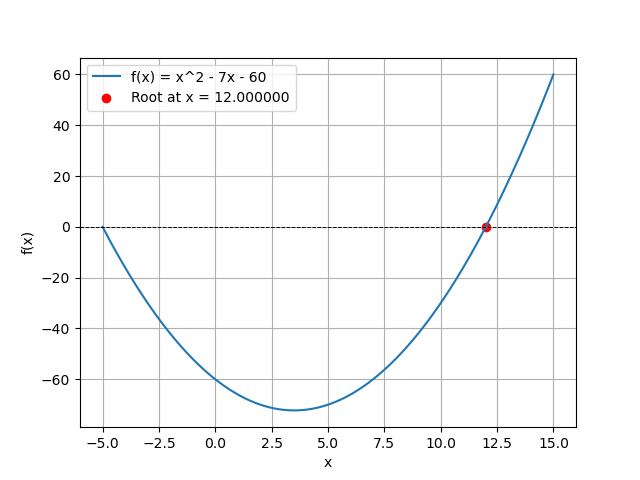
\includegraphics[width=\columnwidth]{figs/Figure_1.png}
	\end{figure}
	
\end{document}  
